%% USPSC-Cap2-Desenvolvimento.tex 

% ---
% Este capítulo, utilizado por diferentes exemplos do abnTeX2, ilustra o uso de
% comandos do abnTeX2 e de LaTeX.
% ---

\chapter{Desenvolvimento}\label{cap_exemplos}

\section{Revisão sistemática}
O estudo de Revisão Sistemática da Literatura seguiu as recomendações Preferred Reporting Items for Systematic Reviews and Meta-Analisys – PRISMA.
Foram buscados os termos: “patent mining”, “patent”, “random forest”, “machine learning” - nas seguintes bases de dados: Periodicos CAPES, Microsoft research, Semantic Scholar e Google Scholar. O intervalo de publicação dos artigos selecionados estão entre 2012 a 2020 e restrito a somente artigos escritos em inglês.

\section{Descrição do objeto de estudo}
Foi realizado a extração de dados de documentos de patentes no site Free Patents Online - FPO (https://www.freepatentsonline.com/). Este site contem os dados dos documentos de patentes de forma pública.

\section{Delineamento da pequisa}
Foi buscado o termo “agronomy” e filtrado para somente documentos de patentes registrados nos Estados Unidos. Foi totalizado 12906 patentes, dos quais selecionamos uma amostragem das 200 primeiras patentes. Construímos uma aplicação de webscraping na linguagem Python para realizar a extração dos dados de documentos de patentes.  Os dados extraídos foram armazenados em um banco de dados.

\section{Procedimentos específicos}

\subsection{Extração dos dados}
A aplicação de webscraping dos dados de documentos de patentes foi escrita na linguagem de programação Python, com uso das bibliotecas \textit{requests} e \textit{BeautifulSoup}. Essa aplicação é modular o suficiente para que seja definido quantos documentos de patentes terão suas informações extraídas, como também quais informações serão extraídas, como demonstrado na figura \ref{webscraping_flow_image}. Os dados são organizados na forma de tabela e armazenado em um pequeno banco de dados feito em \textit{SQLite}.

\begin{figure}[ht!]
	\centering
	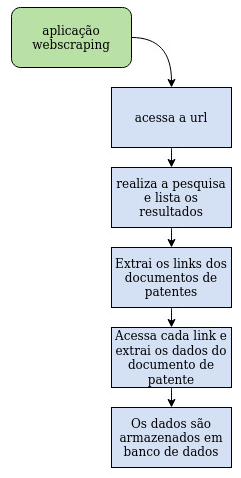
\includegraphics[scale=0.5]{imagens/tcc_webscraping.jpg}
	\caption{Fluxo de captura dos dados de documentos de patente 
			 \label{webscraping_flow_image}}
\end{figure}


\subsection{Construção do dicionario}
A construção do dicionario que será utilizado no projeto é composto pelas seguintes etapas, figura \ref{dicionario_flow_image}, geração de um corpora de documentos de patentes, pre processamento do corpora, obtenção da matriz de documento-termo (Document-Term Matrix – DTM) e aplicação do modelo Latent Dirichlet allocation (LDA). A partir dos tópicos apresentados pelo resultado do LDA, são adicionados ao tópicos, palavras relacionadas, tais como sinônimos, hiperônimos e hipônimos através do banco de dados wordnet.

\begin{figure}[ht!]
	\centering
	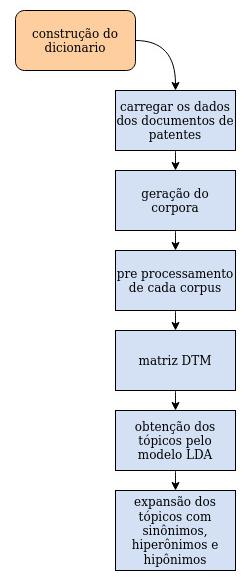
\includegraphics[scale=0.5]{imagens/tcc_dicionario.jpg}
	\caption{Fluxo de criação do dicionario
			 \label{dicionario_flow_image}}
\end{figure}

\section{Validação do dicionario}
A avaliação do dicionario obtido, consiste em observar se o valor k utilizado para geração de tópicos conseguiu separar adequadamente os assuntos contidos no corpora.



